\section{Method}

\subsection{Collection}

    \subsubsection{Collection of device activity data}

        All device activity is collected using the automated time tracker ActivityWatch~\cite{bjareholt_activitywatch_2020-1}.

        ActivityWatch collects data through modules called watchers which report to the ActivityWatch server. It comes with two watchers by default:

        \begin{itemize}
            \item aw-watcher-window, tracks the active window and its title
            \item aw-watcher-afk, tracks if the user is active or not by observing input device activity
        \end{itemize}

        We've also built a custom watcher, aw-watcher-input, to track metrics of mouse and keyboard activity. It tracks by listening to mouse and keyboard events and records the distance\footnote{in pixels} the mouse moves and number of clicks (but not which key was clicked). Every second this is bundled into an event, the values are reset, and then it continues with the next event. It was inspired by similar functionality in Andrej Karpathy's ulogme~\cite{ulogme}.

        A limitation that we have to consider is that the window watcher uses a polling method to track the active window, with a default poll time of 1 second. This means that we can't rely on the timestamps to mark the exact time the window became active/inactive.

        The data from ActivityWatch is processed and categorized such that the resulting data has the 3 columns \mintinline{python}{start, end, category}. The category is determined by a regular expression that matches on window titles and URLs, such as \mintinline{python}{github.com}.

    \subsubsection{Collection of EEG data}

        EEG data was collected during organic device use and under controlled conditions.

        For both conditions, code from the open source eeg-notebooks~\cite{noauthor_neurotechxeeg-notebooks_2020} was adapted to record the raw EEG stream into a CSV file. For the Muse S, muse-lsl~\cite{muse-lsl} was used as the underlying software to handle the connection (which uses Lab Streaming Layer). For the OpenBCI and Neurosity devices, brainflow~\cite{noauthor_brainflow-devbrainflow_2020} was used to handle the connection.

        \paragraph{During organic device use}

            For the organic device use conditions, we primarily used the Muse S due the superior comfort and ease of use compared with the alternatives, making it especially suitable for long recordings.\footnote{A wet electrode cap system was also considered, but ultimately not investigated due to being inconvenient to setup.}

            The subject was then simply asked to go about their usual device activities, often consisting of a mix of work (email, writing prose, writing code) and leisure (watching YouTube, reading Twitter).

        \paragraph{During code vs prose comprehension task}

            For the controlled condition, we ended up using the Muse S as well due to the comfort and ease of setup.

            We implemented the task in eeg-notebooks~\cite{noauthor_neurotechxeeg-notebooks_2020}, which uses previously mentioned libraries for data collection as well as PsychoPy~\cite{peirce_psychopy2_2019} to provide the stimuli.

            The experiment consists of presenting images with code or prose comprehension tasks, as seen in Figure~\ref{fig:codetask} and~\ref{fig:prosetask}.

            \begin{figure}
                \begin{center}
                    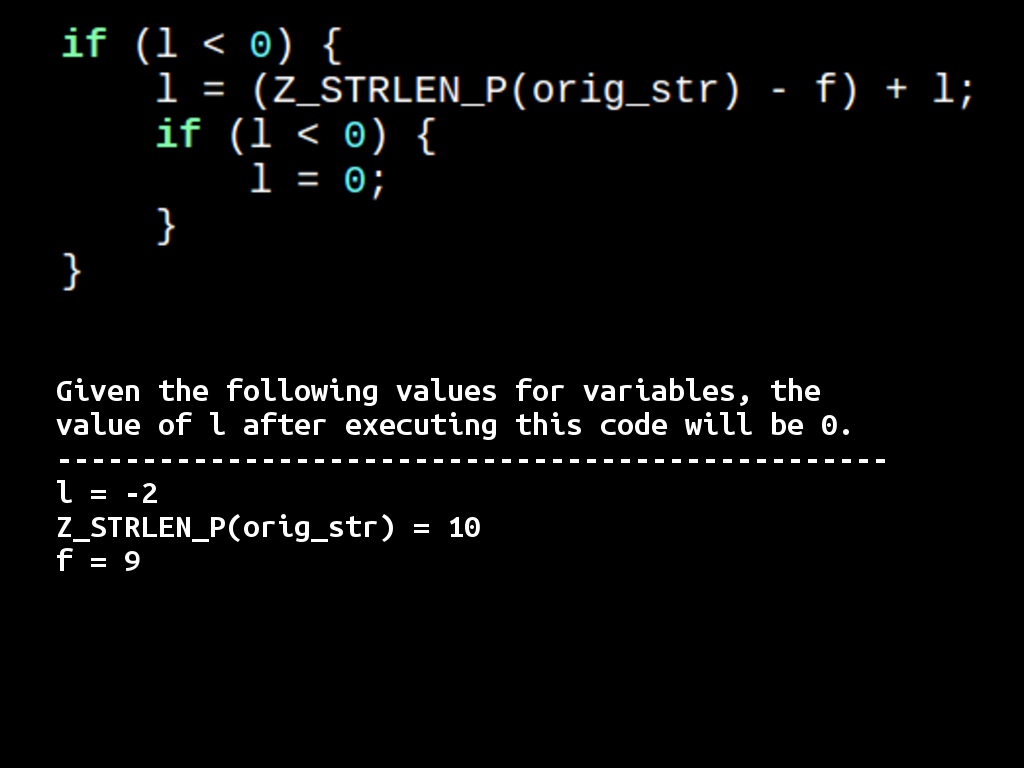
\includegraphics[trim=0 120 0 0,clip,width=100mm]{img/final-1-1.png}
                \end{center}
                \caption{Sample of the code comprehension task}\label{fig:codetask}
            \end{figure}

            \begin{figure}
                \begin{center}
                    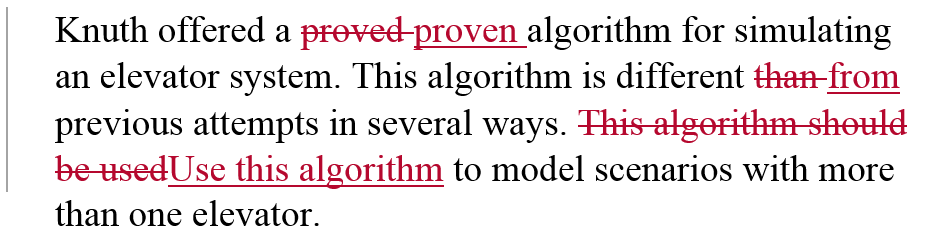
\includegraphics[width=100mm]{img/bugs_1.PNG}
                \end{center}
                \caption{Sample of the prose review task}\label{fig:prosetask}
            \end{figure}

            Before each run, the subject was asked about their gender, age, and software development experience (specifically experience with C/C++). For good measure, we also asked if the subject had consumed caffeine the hours prior to the experiment.

            After these questions we put the devices on and ensure we get good signal by inspecting it in real time with the viewer provided by muse-lsl. The viewer itself does simple bandpass filtering between 3--40Hz, and the signal quality is indicated by the standard deviation of the filtered signal.

        \paragraph{Devices}

            We experimented with several devices but eventually settled on the Muse S. The motivation for choosing the Muse S was mainly due to comfort and ease of use. The other devices considered included the OpenBCI Cyton (with Ultracortex headset) and the Neurosity Notion DK1.

            The Muse S is a 4-channel EEG headband with electrodes at TP9, AF7, AF8, and TP10, with the reference electrode at Fpz~\cite{krigolson_choosing_2017}.\footnote{According to the 10--20 system.}

            \begin{widepage}
            \begin{table}
                \begin{tabular}{llccc}
                    \toprule
                    Manufacturer
                    & Device
                    & Channels
                    & Sampling rate
                    & Comfort
                    \\ 
                    \midrule
                    InteraXon
                    & Muse S
                    & 4
                    & 250Hz
                    & High \\
                 OpenBCI
                    & Cyton (with Ultracortex)
                    & 8
                    & 125--250Hz
                    & Low \\
                 % generously gifted by Neurosity
                 Neurosity
                    & Notion DK1
                    & 8
                    & 250Hz
                    & Medium \\
                  % preordered, arrives in late spring
                  Neurosity
                    & Crown
                    & 8
                    & 250Hz
                    & High? \\
                    \bottomrule
                \end{tabular}
                \caption{Devices used}\label{table:devices}
            \end{table}
            \end{widepage}

            \begin{center}
            \begin{figure}
                \begin{widepage}
                \begin{tabular}{cc}
                    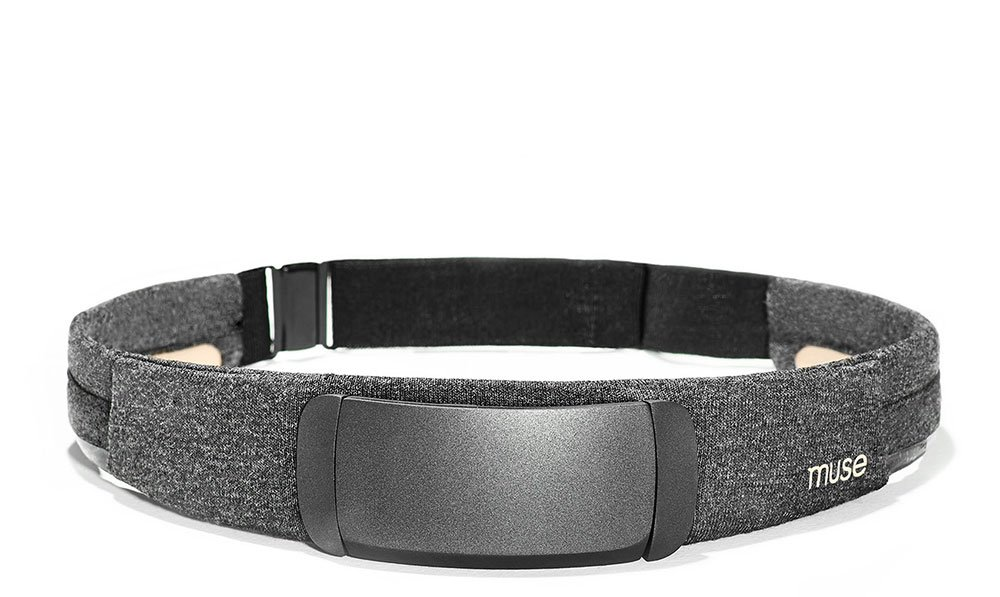
\includegraphics[width=65mm]{img/Muse-S.jpg}
                    & 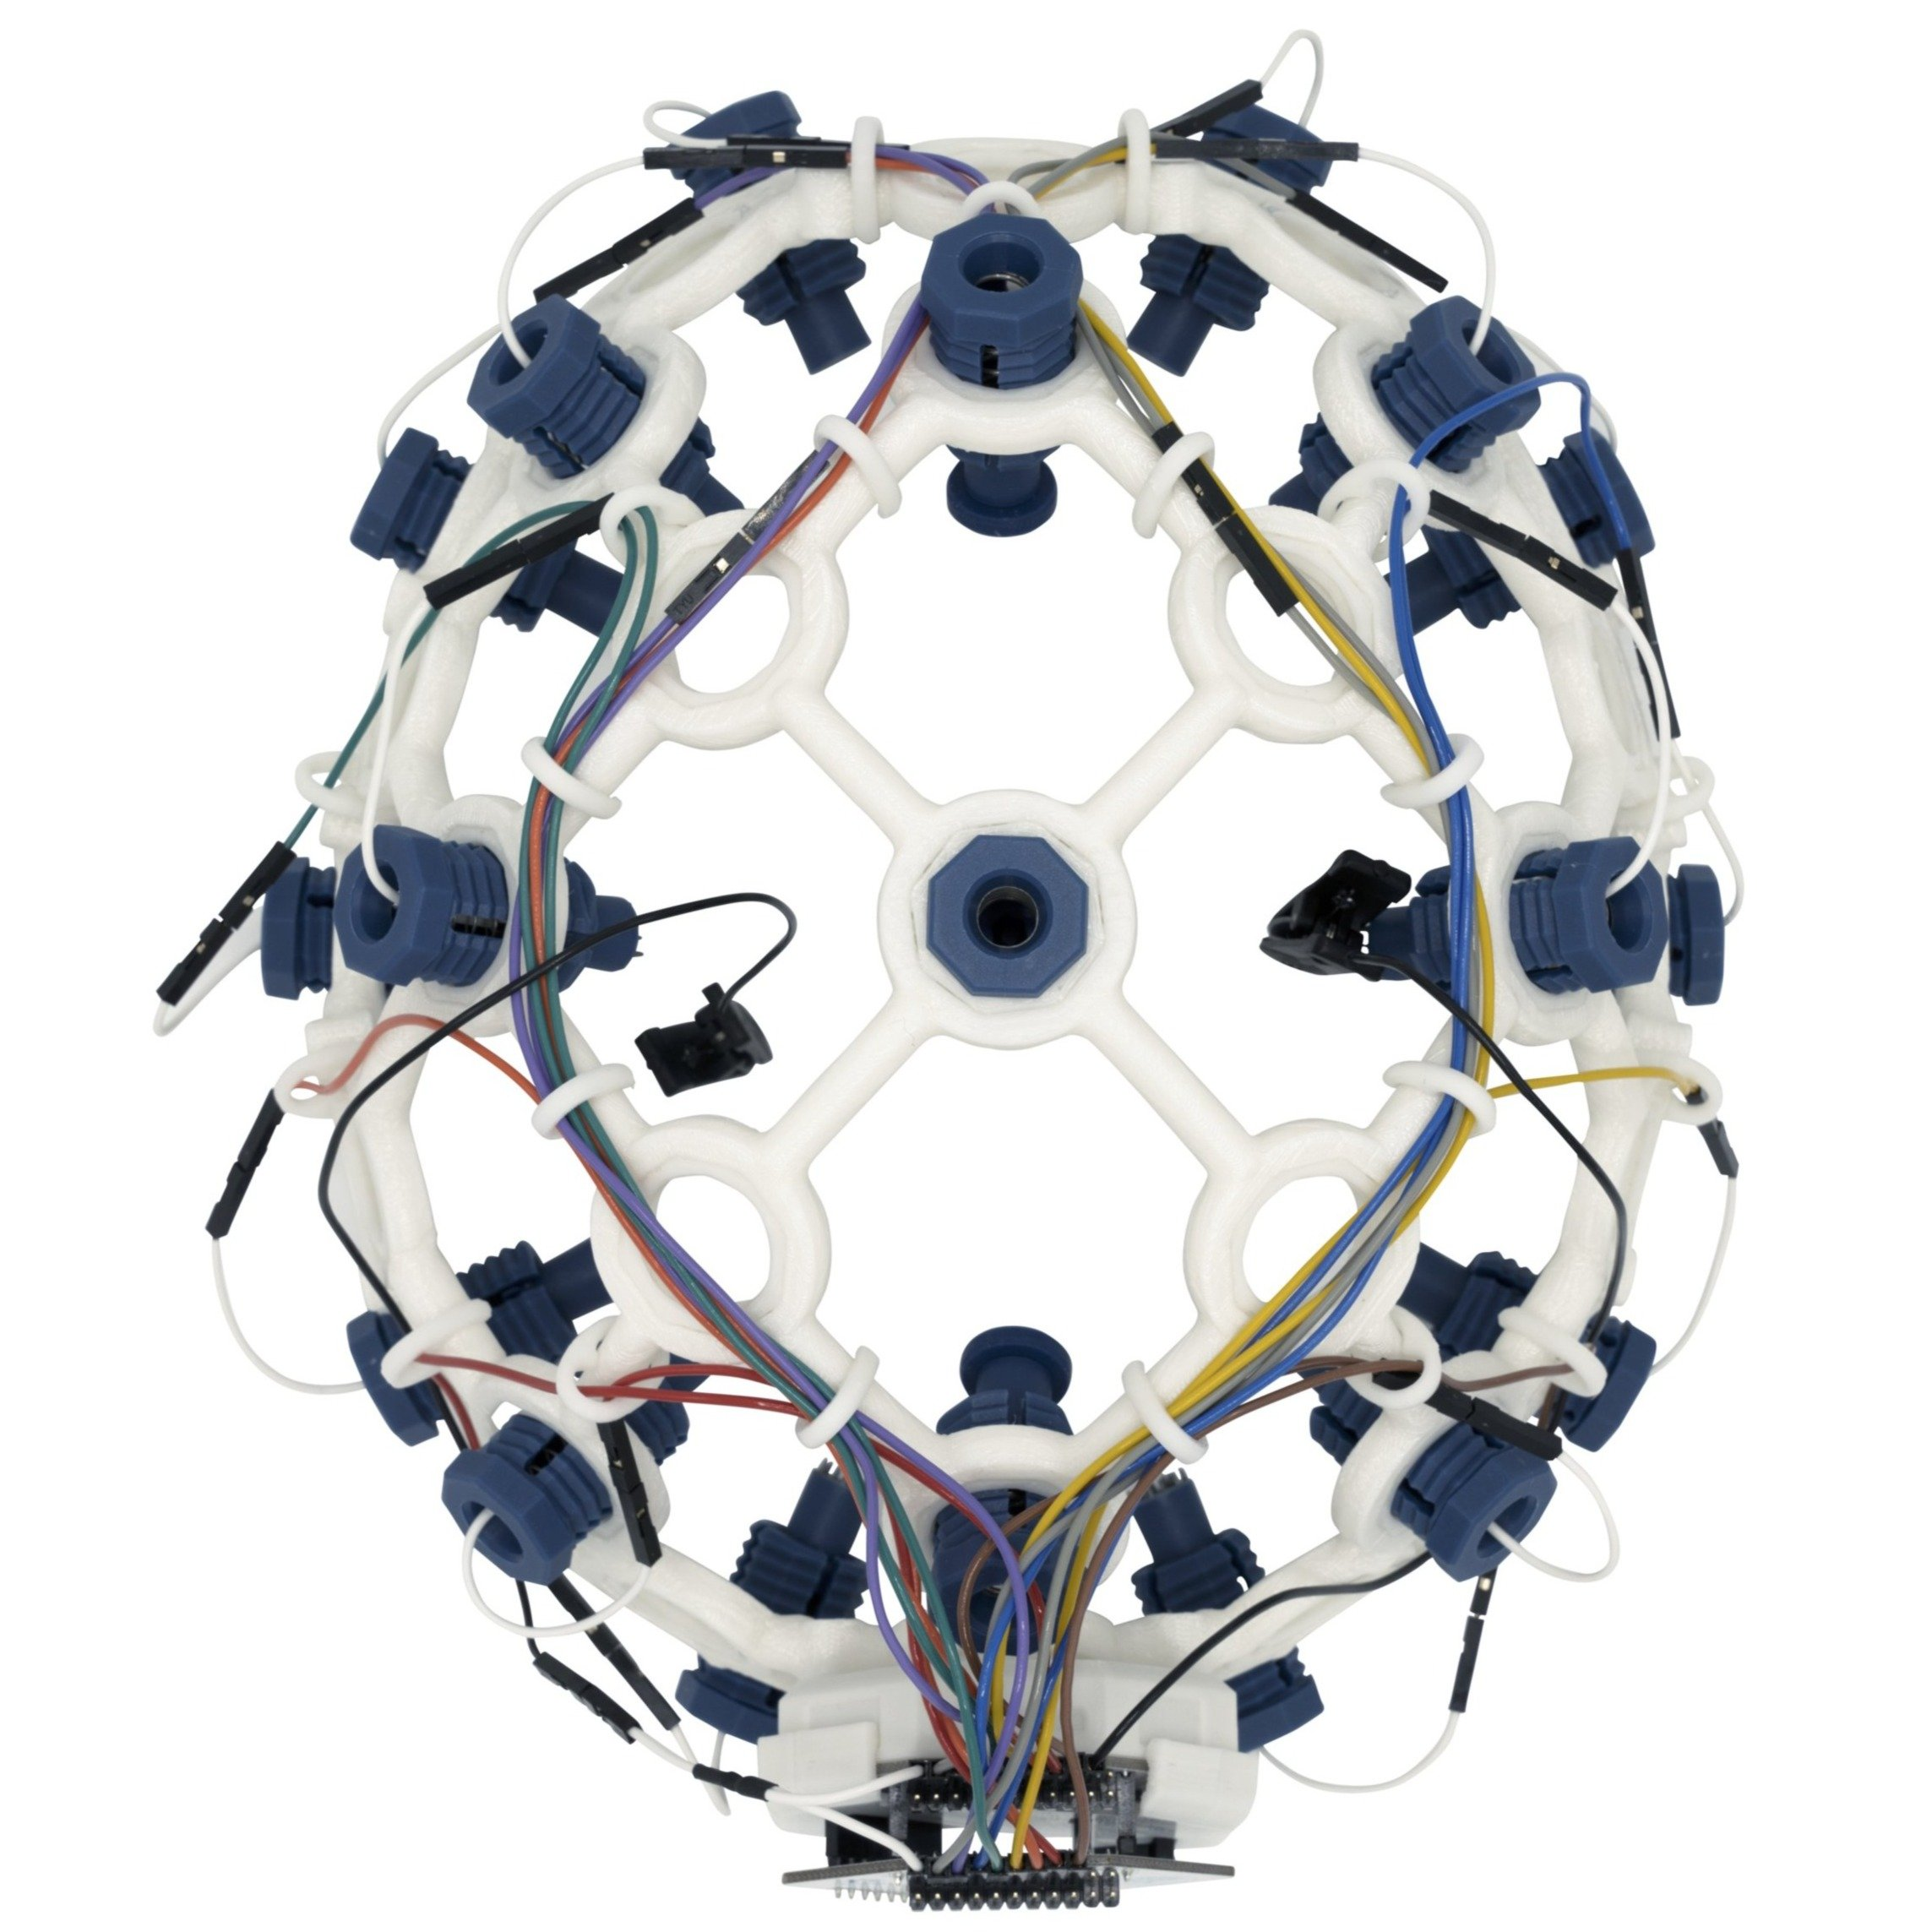
\includegraphics[width=65mm]{img/openbci-cyton.jpg}
                    \\
                    (a) Muse S
                    & (b) OpenBCI Cyton with Ultracortex
                    \\[6pt]
                    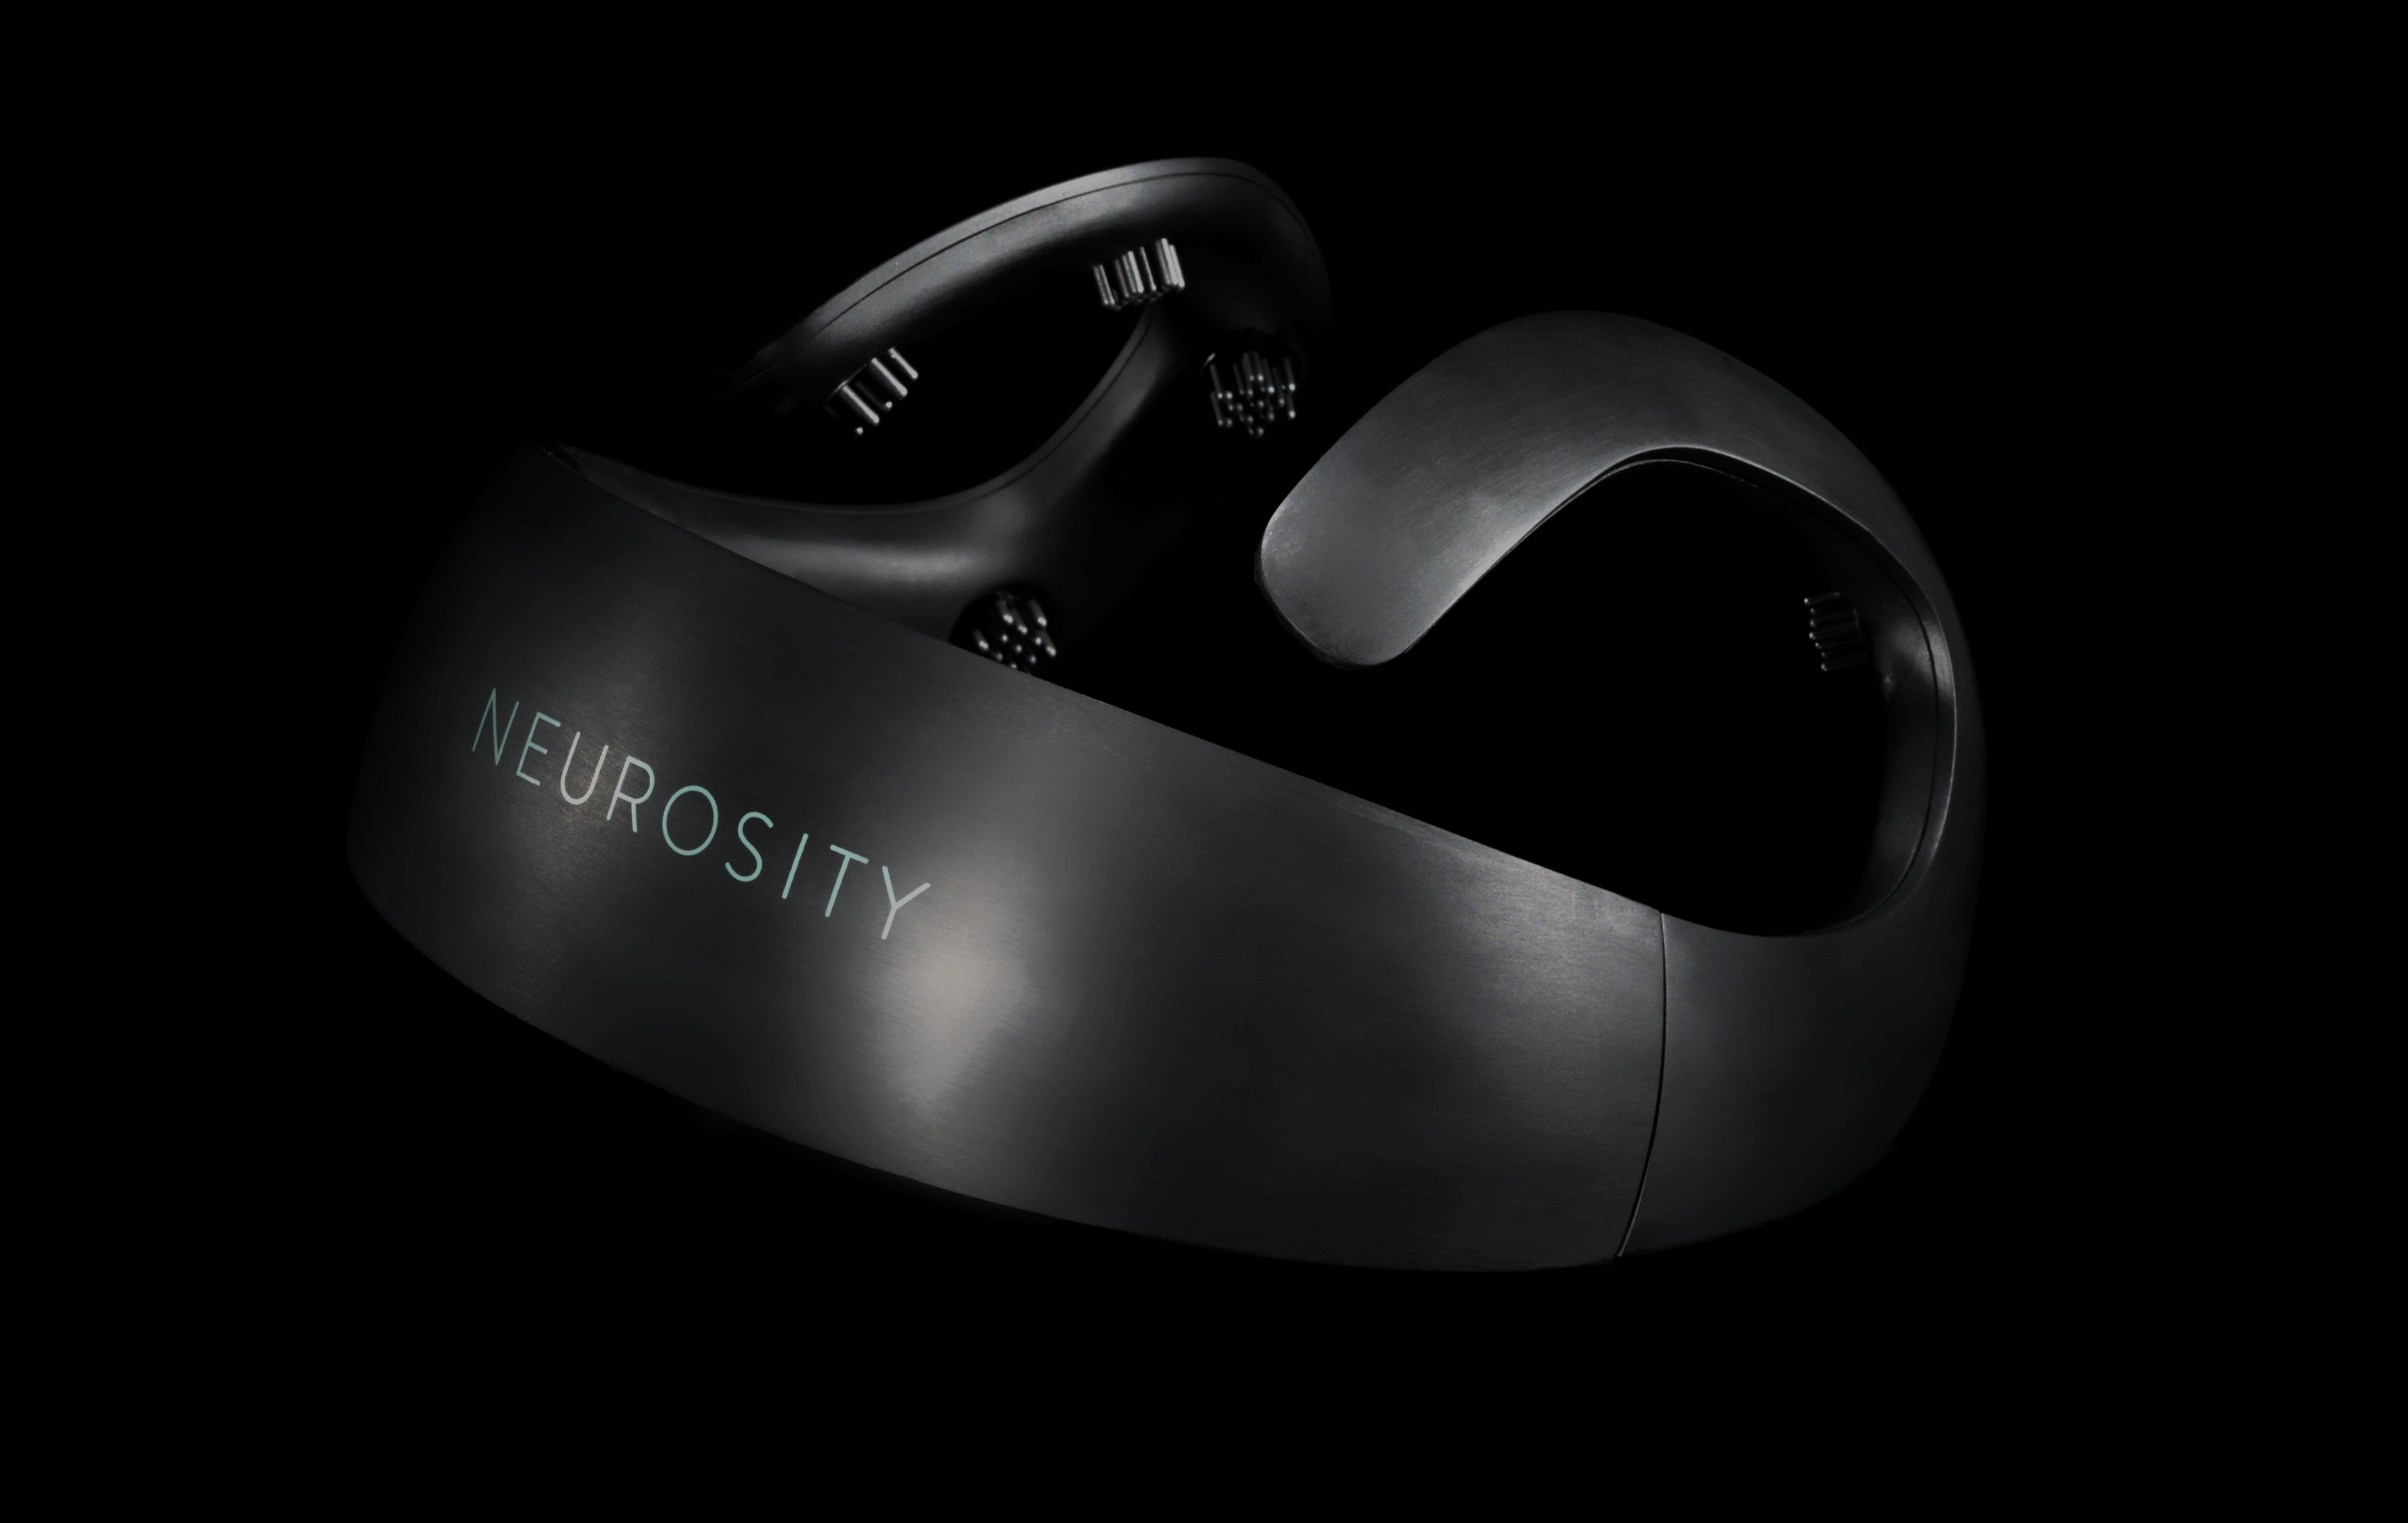
\includegraphics[width=65mm]{img/neurosity-notion.png}
                    & 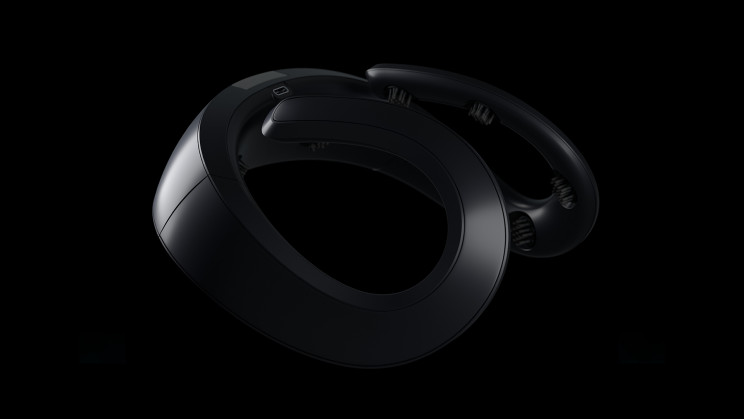
\includegraphics[width=65mm]{img/neurosity-crown.jpg}
                    \\
                    (c) Neurosity Notion DK1
                    & (d) Neurosity Crown
                    \\[6pt]
                \end{tabular}
                \caption{Photos of devices used}
                \end{widepage}
            \end{figure}
            \end{center}

\subsection{Analysis}

    For classification and analysis, we used common open source Python libraries for data analysis, like numpy~\cite{harris2020array}, pandas~\cite{reback2020pandas}, and scikit-learn~\cite{scikit-learn}. In addition, we used less common libraries tailored specifically for working with EEG data, such as MNE~\cite{noauthor_mne-toolsmne-python_2020}, pyriemann~\cite{alexandre_barachant_2020_3715511}, and YASA~\cite{raphael_vallat_raphaelvallatyasa_2020}.

    \subsubsection{Data cleaning}

        For the uncontrolled condition, we align the raw EEG data with the categories assigned by our ActivityWatch script. We split the series into epochs, and reject samples that either:

        \begin{enumerate}
            \item Don't have an assigned class
            \item Have a bad signal quality (as indicated by a high signal variance)
            \item Are too short (due to missing samples)
        \end{enumerate}

        \todo[inline]{List how many epochs are rejected by each cleaning step}

    \subsubsection{Feature engineering}

        \paragraph{Bandpower}

            Bandpower features are simple and commonly used in EEG research for many tasks, including the paper by Fucci et al we seek to improve upon~\cite{fucci_replication_2019}. As a reference, we implemented classifiers which solely used bandpower features as input, to gain information of how much any improvement from classifier performance is likely due to better EEG equipment versus how much is due to from improved analysis methods.

            To compute this feature, we utilized the bandpower function provided by YASA~\cite{raphael_vallat_raphaelvallatyasa_2020}. The implementation estimates the power spectral density using Welch's method for each channel, and bins them by their associated frequency band.

            To further enrich our feature vector, we can use ratios between two frequency bands.

        \subsubsection{Riemannian geometry}

            The \improvement{according to whom?}{state of the art in many EEG classification tasks} involves the use of Riemannian geometry. For this, we used the open source pyriemann library by Alexandre Barachant\footnote{First author of the original paper to apply Riemannian geometry to EEG~\cite{barachant_classification_2013}}.

    \subsubsection{Neural Networks}

        One of the classifiers we want to train is a neural network. We use braindecode~\cite{schirrmeister_deep_2017}\cite{noauthor_braindecodebraindecode_2021}, a neural network toolbox for EEG data that uses PyTorch and integrates it with scikit-learn through skorch.

        The networks provided by braindecode are\ldots

    \subsubsection{Cross Validation}

        We use LORO (``Leave-One-Run-Out'') cross-validation, a variation of LOGO (``Leave-One-Group-Out''), in order to ensure the samples used in validation are using subjects or tasks that are unseen in training.

        We attempt both out-of-subject validation and out-of-task validation in order to estimate the ability of the classifiers to generalize across subjects and tasks.
